\documentclass{article}
\usepackage[utf8]{inputenc}
\usepackage{pgfplots}
\usepackage{amsmath}
\usepackage{amssymb}
\usepackage{tikz}
\usepackage{pdflscape}


\begin{document}

\begin{landscape}
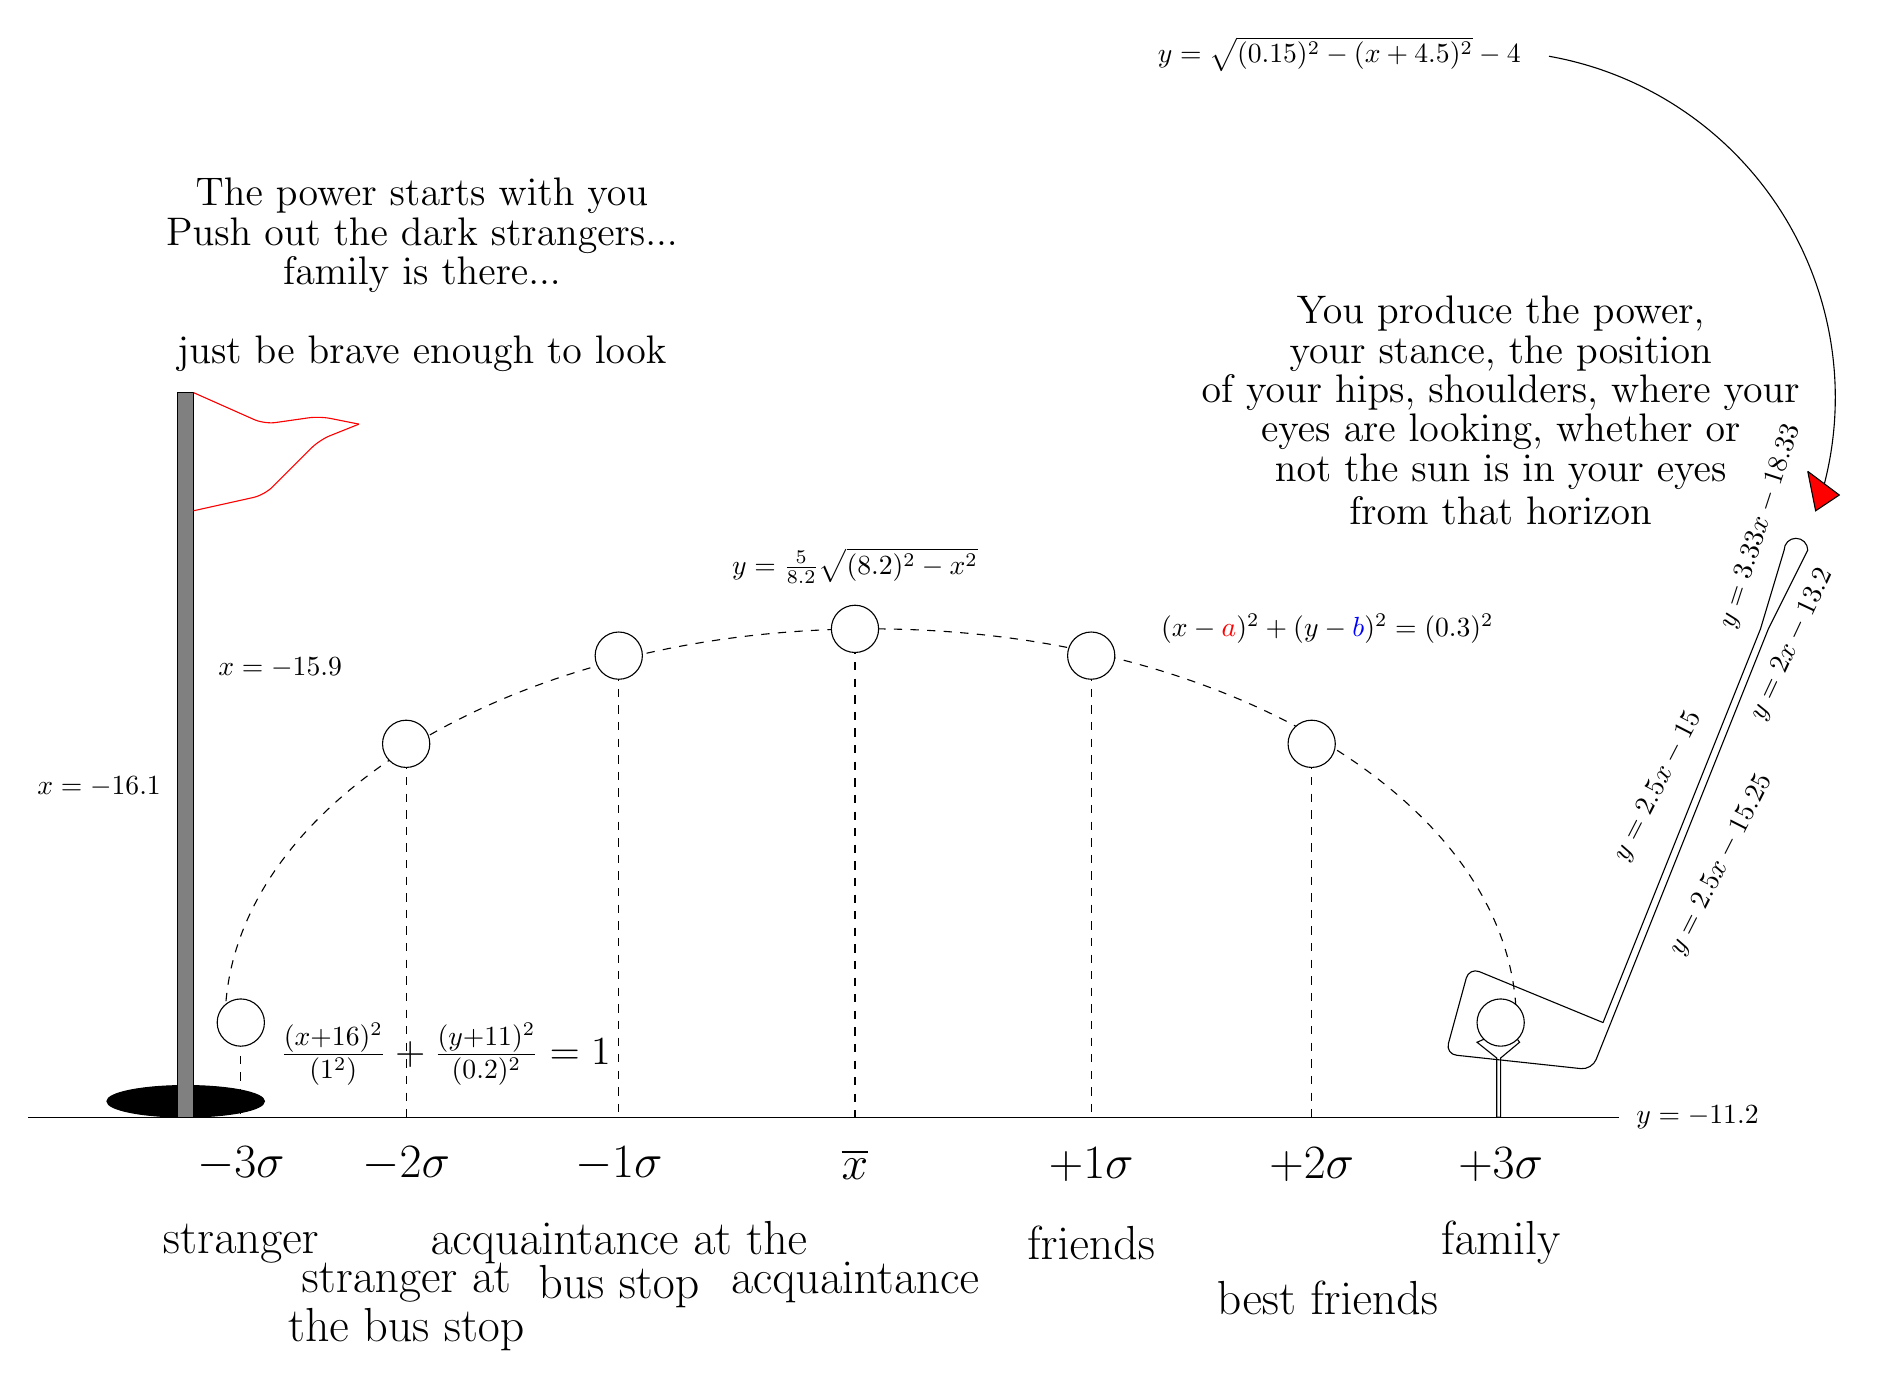
\begin{tikzpicture}


%golf long stick part
\draw (2,-10)--(4,-5); % left side
\draw (2.1,-10)--(4.1,-5); %right side


%cone shaped handle on top of long stick part
\draw (4,-5)--(4.3,-4);  %left side of 'cone'  handle
\draw (4.1,-5)--(4.6,-4); %right side of 'cone'  handle
\draw (4.6,-4) arc (0:180:0.15); % arc on top of handle


%starting golf ball on tee
\draw (0.487,-10.212)--(0.4,-10.25)--(0.65,-10.45)--(0.65,-11.2); % left side of tee
\draw (0.912,-10.212)--(0.94,-10.25)--(0.7,-10.45)--(0.7,-11.2)--(0.65,-11.2); % right side of tee + bottom


%golf club part
\draw [rounded corners] (2.1,-10)--(1.86,-10.6)--(0,-10.4)--(0.3,-9.3)--(2,-10); 


%golf hole as a whole
\draw [fill = black] (-16,-11) ellipse (1cm and 0.2cm); %golf hole
\draw [fill = gray] (-15.9,-11.2)--(-16.1,-11.2)--(-16.1,-2)--(-15.9,-2)--(-15.9,-11.2); % flag pole

\draw [rounded corners, color = red] (-15.9,-2)--(-15,-2.4)--(-14.3,-2.3)--(-13.8,-2.4); %top side of flag
\draw [rounded corners, color = red] (-15.9,-3.5)--(-15,-3.3)--(-14.3,-2.6)--(-13.8,-2.4); %bottom side of flag


%vertical lines for emperical rule
\draw [dashed] (-7.5,-5)--(-7.5,-11.2) node at(-7.5,-11.8){\LARGE$\overline{x}$}; %mean line
\draw [dashed] (-4.5,-5.34)--(-4.5,-11.2) node at(-4.5,-11.8){\LARGE$+1\sigma$};
\draw [dashed] (-10.5,-5.34)--(-10.5,-11.2) node at(-10.5,-11.8){\LARGE$-1\sigma$};
\draw [dashed] (-13.2,-6.46)--(-13.2,-11.2) node at(-13.2,-11.8){\LARGE$-2\sigma$};
\draw [dashed] (-1.7,-6.46)--(-1.7,-11.2) node at(-1.7,-11.8){\LARGE$+2\sigma$};
\draw [dashed] (-15.3,-10)--(-15.3,-11.2) node at(-15.3,-11.8){\LARGE$-3\sigma$};
\node at(0.7,-11.8){\LARGE$+3\sigma$};



\draw [dashed] (0.9,-10) arc (0:180:8.2cm and 5cm); %dotted golf ball trajectory
\draw [fill = white] (0.7,-10) circle (0.3cm); %starting golf ball
\draw [fill = white] (-1.7,-6.46) circle (0.3cm); %golf ball 1 (from right)
\draw [fill = white] (-4.5,-5.34) circle (0.3cm); %golf ball 2 (from right)
\draw [fill = white] (-7.5,-5) circle (0.3cm); %golf ball 3 (from right)
\draw [fill = white] (-10.5,-5.34) circle (0.3cm); %golf ball 4 (from right)
\draw [fill =white] (-13.2,-6.46) circle (0.3cm); %golf ball 5 (from right)
\draw [fill = white] (-15.3,-10) circle (0.3cm); %golf ball 6 (from right)

\node at(-7.5,-4.2){$y=\frac{5}{8.2}\sqrt{(8.2)^2-x^2}$};
\node at(2.7,-7){\rotatebox{62.8}{$y=2.5x-15$}};
\node at(3.5,-8){\rotatebox{63.1}{$y=2.5x-15.25$}};
\node at(4,-3.7){\rotatebox{72}{$y=3.33x-18.33$}};
\node at(4.4,-5.2){\rotatebox{65}{$y=2x-13.2$}};
\node at(-17.1,-7){$x=-16.1$};
\node at(-14.8,-5.5){$x=-15.9$};
\node at(3.2,-11.2){$y=-11.2$};
\node at(-12.7,-10.4){\Large$\frac{(x+16)^2}{(1^2)}+\frac{(y+11)^2}{(0.2)^2}=1$};
\node at(-1.5,-5){$(x-\textcolor{red}{a})^2+(y-\textcolor{blue}{b})^2=(0.3)^2$};



\draw (-18,-11.2)--(2.2,-11.2); %line representing ground/ emperical rule

%sayings underneath the separations
\node at(0.7,-12.8){\LARGE family};
\node at(-1.5,-13.5){\LARGE best friends};
\node at(-4.5,-12.8){\LARGE friends};
\node at(-7.5,-13.3){\LARGE acquaintance};
\node at(-10.5,-12.8){\LARGE acquaintance at the};
\node at(-10.5,-13.35){\LARGE bus stop};
\node at(-13.2,-13.3){\LARGE stranger at};
\node at(-13.2,-13.9){\LARGE the bus stop};
\node at(-15.3,-12.8){\LARGE stranger};

%sayings above golf club
\node at(0.7,-1){\Large You produce the power,}; 
\node at(0.7,-1.5){\Large your stance, the position};
\node at(0.7,-2){\Large of your hips, shoulders, where your};
\node at(0.7,-2.5){\Large eyes are looking, whether or};
\node at(0.7,-3){\Large not the sun is in your eyes};
\node at(0.7,-3.5){\Large from that horizon};

%sayings above flag pole
\node at(-13,0.5){\Large The power starts with you};
\node at(-13,0){\Large Push out the dark strangers...};
\node at(-13,-0.5){\Large family is there...};
\node at(-13,-1.5){\Large just be brave enough to look};


\draw (4.8,-3.2) arc (-15:80:4.4cm);%arc for the red arrow
\draw [fill = red] (4.6,-3)--(5,-3.3)--(4.7,-3.5)--(4.6,-3); %red arrow for small arc
\node at(-1.35,2.3){$y=\sqrt{(0.15)^2-(x+4.5)^2}-4$};



\end{tikzpicture}
\end{landscape}


\end{document}